%\documentclass{cwpreport} % for review/editing/polishing
%\linespread{1.5}           % for review/editing/polishing
\documentclass[onecolumn]{cwpreport} % for final draft
%\documentclass[]{article}

% Packages used by default CWP reports built by M8R
\usepackage{times,natbib,amsmath,graphicx,color,amssymb,amsbsy,lineno,setspace,algorithm2e,lipsum,hyperref,appendix}

\usepackage{xcolor}

% Specific paper formatting for CWP report
\setlength{\paperwidth}{8.5in}
\setlength{\paperheight}{11.0in}
\setlength{\topmargin}{-0.25in}
\setlength{\textheight}{8.75in}
\setlength{\textwidth}{6.5in}
\setlength{\oddsidemargin}{+.015625in}
\setlength{\evensidemargin}{+.015625in}


\title{Accoppiamento FEM/BEM: implementazione delle condizioni di dominio aperto nel codice FEM 2D
elettrostatico \thanks{Progetto realizzato nell'ambito del corso \textit{Computational Electromagnetics}}} 

\author[Matteo Morana]{Matteo Morana \\
Master Student in Mathematical Engeneering at Politecnico di Milano \\ email matteo.morana@mail.polimi.it} 

\begin{document}


\maketitle



\begin{abstract}
\lipsum[2]
\end{abstract}


\begin{keywords}
Keyword1, Keyword2, Keyword3 
\end{keywords}


\section{Introduction}

A classic example of FEM/BEM coupling in an electrostatic problem is the computation of the electric field generated by a parallel-plate capacitor. In a simulation of this type, it is often useful to visualize not only the behavior of the field inside the capacitor, but also outside it. In Physics II courses, the external field is usually assumed to be zero; in reality, due to edge effects, it is not negligible, and in some applications it can play a significant role. This is the main motivation for analyzing in greater detail the behavior of the electric field in such a problem.

In this project, we consider the relatively simple case of a parallel-plate capacitor (see the reference figure). Besides the charges present on the plates, no other sources are considered in the surrounding space. The differential equation to be solved is Maxwell's first law ~\eqref{eq:prima_legge_maxwell} in its simplified electrostatic form ~\eqref{eq:prima_legge_maxwell_semplificata}, expressed by treating the electric field as the gradient of the potential ~\eqref{eq:prima_legge_maxwell_semplificata_potenziale}.

\begin{equation}
	\nabla \cdot D = \rho
\label{eq:prima_legge_maxwell}
\end{equation}

\begin{equation}
	\nabla \cdot E = 0
\label{eq:prima_legge_maxwell_semplificata}
\end{equation}

\begin{equation}
	\Delta V = 0
\label{eq:prima_legge_maxwell_semplificata_potenziale}
\end{equation}

A well-known first approach consists in using the Finite Element Method (FEM). One defines a domain large enough to contain the capacitor and imposes a zero potential on its boundary, assuming that at a sufficiently large distance the potential effectively tends to zero. However, this method has some drawbacks: it requires very large domains and therefore large meshes, resulting in increased computational time. Moreover, the mesh resolution must be uniform inside and outside the capacitor, even though the quality required to obtain an accurate result is not the same in the two regions. Computing the external field with FEM therefore leads to significant computational waste, and in any case the potential cannot be represented up to infinity, introducing an unavoidable approximation.

The Boundary Element Method (BEM), on the other hand, offers a more efficient solution to the problem. By reducing the dimension of the domain by one order, it allows substantial computational advantages. By its nature, BEM enables the accurate computation of the unknown variable at any internal point of a domain, solving the problem only on its boundary (fig.). BEM is also applicable to very large or unbounded domains (fig.), provided that the asymptotic behavior of the potential is known a priori and that it converges as $1/r^2$. In such cases, BEM can correctly represent the behavior at infinity without introducing artificial approximations.

The goal of this work is therefore to combine FEM and BEM to obtain more accurate results at lower computational cost. The idea is to use FEM to determine the solution accurately inside the capacitor and employ BEM to extend it outward to infinity in an exact manner. The coupling mechanism between the two methods will be described in detail in the dedicated section.

\section{Coupled}
\subsection{FEM formulation}
In this section we derive the FEM formulation for our problem, we do not perform the FEM as usual, since we need to achieve a specific formulation in order to couple FEM and BEM.


The problem to solve is ~\eqref{eq:problema_laplaciano}

\begin{equation}
    \Delta u = 0 \quad \text{in } \Omega.
\label{eq:problema_laplaciano}
\end{equation}

Let's rewrite the problem in the weak formulation ~\eqref{eq:weak_formulation}


\begin{equation}
\begin{aligned}
&\text{Find } u \in H^1(\Omega) \quad \text{s.t}
&\int_{\Omega} \nabla u \cdot \nabla v \, dx  \, -\int_{\partial\Omega} \frac{\partial u}{dn}v\,ds = 0
\qquad \forall v \in H_{g}^1(\Omega) := \{v \in H^1  \text{ s.t. } v ... \}
\end{aligned}
\label{eq:weak_formulation}
\end{equation}

We did not write boundary conditions for the problem. this is because we have neither Dirichlet nor Neumann boundary conditions; we have a relation between $u$ and $\frac{\partial u}{dn}$ thanks to the BEM method. So, for now, let's write the problem in this way without imposing any bcs.

Now we consider that to have equation ~\eqref{eq:weak_formulation} verified $\forall v$ it's sufficient to verify for each element of the base of $H^1$. We also discretize the problem and so do not solve the problem for $v \in H^1$ but for $v_h \in V_h \subset H^1$. These consideration leads to $N_h$ equations, where $N_h$ is the dimension of the space $V_h$. Now we observe that $u \in V_h$ therefore we can write $u$ as $\sum_{j=1}^{N_h} u_jv_j$ where $v_j$ are the basis of $V_h$. We can now write the problem as in ~\eqref{eq:discrete_formulation} where $v_i$ forms the base of the $V_h$ space. We can see ~\eqref{eq:discrete_formulation} as a system of $N_h$ equations in $N_h$ unknowns which are $u_j$. If we achieve $u_h$ we can perform $\sum_{j=1}^{N_h} u_jv_j$ and obtain $u \in V_h$ which is the solution of our problem.

\begin{equation}
\begin{aligned}
&\text{Find } u_j \,,\, j = 1,...,N_h\quad \text{s.t}
&\int_{\Omega} \nabla (\sum_{j=1}^{N_h} u_jv_j) \cdot \nabla v_i \, dx  \, -\int_{\partial\Omega} \frac{\partial (\sum_{j=1}^{N_h} u_jv_j)}{dn}v_i\,ds = 0
\qquad \forall v_i \,,\, i = 1,...,N_h
\end{aligned}
\label{eq:discrete_formulation}
\end{equation}

With this notation we lose information about the normal derivative since we can rearrange the term and take out $u_j$ that are constant from the derivative. So to mantain a $\frac{\partial u}{dn}$ we consider that $\frac{\partial u}{dn}$ can be written as $\sum_{j=1}^{N_h} x_jv_j$ where $v_j$ are the basis of $V_h$ and $x_j$ are coefficient. In fact since we can select the space $V_h$, it's possibile to choose a space who garantee that both $u$ and $\frac{\partial u}{dn}$ are element of this space an therefore written as a proper linear combination of the basis of the space. We rewrite ~\eqref{eq:discrete_formulation} as ~\eqref{eq:discrete_formulation_2}, in the new formulation $x_i$ represents the coefficient to find to achieve the normal derivative. To highlight the meaning of $x_i$ we report also ~\eqref{eq:discrete_formulation_3} in which $x_i$ are called $\frac{\partial u_i}{dn}$, is important to pay attention to this notation because we are not appling the normal derivative operator to $u_i$ which is a coefficient, and the operator would not be meaningful since the operation would result in 0. We are just denoting the coefficient with the symbol $\frac{\partial u_i}{dn}$

\begin{equation}
\begin{aligned}
&\text{Find } u_j ,x_j \,,\, j = 1,...,N_h\quad \text{s.t}
&\int_{\Omega} \nabla (\sum_{j=1}^{N_h} u_jv_j) \cdot \nabla v_i \, dx  \, -\int_{\partial\Omega} (\sum_{j=1}^{N_h} {\color{red}x_j}v_j)v_i\,ds = 0
\qquad \forall v_i \,,\, i = 1,...,N_h
\end{aligned}
\label{eq:discrete_formulation_2}
\end{equation}


\begin{equation}
\begin{aligned}
&\text{Find } u_j,x_j \,,\, j = 1,...,N_h\quad \text{s.t}
&\int_{\Omega} \nabla (\sum_{j=1}^{N_h} u_jv_j) \cdot \nabla v_i \, dx  \, -\int_{\partial\Omega} (\sum_{j=1}^{N_h} {\color{red}\frac{\partial u_j}{dn} }v_j)v_i\,ds = 0
\qquad \forall v_i \,,\, i = 1,...,N_h
\end{aligned}
\label{eq:discrete_formulation_3}
\end{equation}


\begin{equation}
\begin{aligned}
&\text{Find } u_j,x_j \,,\, j = 1,...,N_h\quad \text{s.t}
&\int_{\Omega}\sum_{j=1}^{N_h} ({\color{blue} u_j}  {\color{green} \nabla v_j \cdot \nabla v_i})  \, dx  \, -\int_{\partial\Omega} (\sum_{j=1}^{N_h} {\color{red}\frac{\partial u_j}{dn} }{\color{green}v_jv_i})\,ds = 0
\qquad \forall v_i \,,\, i = 1,...,N_h
\end{aligned}
\end{equation}


\begin{equation}
\begin{aligned}
&\text{Find } u_j,x_j \,,\, j = 1,...,N_h\quad \text{s.t}
&\sum_{j=1}^{N_h} ({\color{blue} u_j}  {\color{green}\int_{\Omega} \nabla v_j \cdot \nabla v_i\, dx})    \, - (\sum_{j=1}^{N_h} {\color{red}\frac{\partial u_j}{dn} }{\color{green}\int_{\partial\Omega}v_jv_i\,ds}) = 0
\qquad \forall v_i \,,\, i = 1,...,N_h
\end{aligned}
\end{equation}


Doing some transformation we can rewrite the problem as ~\eqref{eq:discrete_formulation_4}

\begin{equation}
\begin{aligned}
\text{Find } u,\frac{\partial u}{\partial n} \text{ s.t. } \quad
&{\color{green} S_i}\, {\color{blue} u} 
- 
{\color{green} T_i}\,
{\color{red} \frac{\partial u}{\partial n}} 
= 0 \qquad \forall v_i, \quad i = 1, \dots, N_h \quad \text{where:}
\end{aligned}
\label{eq:discrete_formulation_4}
\end{equation} 

\begin{equation}
A_i 
= 
\begin{bmatrix}
\int_{\Omega}\nabla v_1 \cdot \nabla v_i &
\int_{\Omega}\nabla v_2 \cdot \nabla v_i &
\dots &
\int_{\Omega}\nabla v_{N_h} \cdot \nabla v_i
\end{bmatrix}
\end{equation}


\begin{equation}
\mathbf{u} = 
\begin{bmatrix}
u_1 & u_2 & \dots & u_{N_h}
\end{bmatrix}^T,
\end{equation}

\begin{equation}
T_i =
\begin{bmatrix}
\int_{\partial\Omega}v_1 v_i &
\int_{\partial\Omega}v_2 v_i &
\dots &
\int_{\partial\Omega}v_{N_h} v_i &
\end{bmatrix}
\end{equation}



\begin{equation}
\frac{\partial \mathbf{u}}{\partial n} =
\begin{bmatrix}
\frac{\partial u_1}{\partial n} &
\frac{\partial u_2}{\partial n} &
\dots &
\frac{\partial u_{N_h}}{\partial n}
\end{bmatrix}^T.
\end{equation}


Visualize the $N_h$ equation as a system we can write ~\eqref{eq:discrete_formulation_5} 

\begin{equation}
\begin{aligned}
&\text{Find } u,\frac{\partial u}{\partial n} \quad \text{s.t}
&{\color{green}S}{\color{blue}u}  \, - {\color{green}T}{\color{red}\frac{\partial u}{dn}} = 0
\end{aligned}
\label{eq:discrete_formulation_5}
\end{equation}
%% ------------------------------------------------------------

\subsection{BEM formulation}
In this section we derive the BEM formulation for our problem. The key idea behind BEM is to reformulate the problem defined on $\Omega$ as an equivalent problem defined only on the boundary $\partial\Omega$, reducing the dimensionality of the problem.

The starting point is the fundamental solution of the Laplace operator. We define $G(x,y)$ as the function satisfying

\begin{equation}
    \Delta_x G(x,y) = -\delta(x-y) \quad \text{in } \mathbb{R}^d,
\label{eq:fundamental_solution}
\end{equation}

where $\delta$ is the Dirac delta distribution and $d$ is the space dimension. The explicit expression of $G$ is:

\begin{equation}
G(x,y) = 
\begin{cases}
-\dfrac{1}{2\pi} \log |x - y| & \text{if } d = 2, \\[6pt]
\dfrac{1}{4\pi |x - y|} & \text{if } d = 3.
\end{cases}
\label{eq:green_function}
\end{equation}

\subsubsection{Green's third identity}
Let $u \in H^1(\Omega)$ be a solution of~\eqref{eq:problema_laplaciano}. Applying Green's second identity to $u$ and $G(\cdot, y)$ for a fixed $y \in \Omega$ yields the \textit{representation formula}~\eqref{eq:representation_formula}:

\begin{equation}
u(y) = \int_{\partial\Omega} G(x,y)\, \frac{\partial u}{\partial n}(x)\, ds_x 
\,-\, \int_{\partial\Omega} \frac{\partial G}{\partial n_x}(x,y)\, u(x)\, ds_x, 
\qquad \forall y \in \Omega.
\label{eq:representation_formula}
\end{equation}

This formula expresses $u$ at any interior point $y$ solely in terms of the boundary values of $u$ and $\frac{\partial u}{\partial n}$. We define the two integral operators appearing in~\eqref{eq:representation_formula}:

\begin{equation}
(\mathcal{V}\phi)(y) := \int_{\partial\Omega} G(x,y)\, \phi(x)\, ds_x,
\label{eq:single_layer}
\end{equation}

\begin{equation}
(\mathcal{K}\phi)(y) := \int_{\partial\Omega} \frac{\partial G}{\partial n_x}(x,y)\, \phi(x)\, ds_x,
\label{eq:double_layer}
\end{equation}

where $\mathcal{V}$ is called the \textit{single layer operator} and $\mathcal{K}$ is called the \textit{double layer operator}. With this notation,~\eqref{eq:representation_formula} becomes:

\begin{equation}
u(y) = \mathcal{V}\left(\frac{\partial u}{\partial n}\right)(y) - \mathcal{K}(u)(y), \qquad \forall y \in \Omega.
\end{equation}

\subsubsection{Boundary Integral Equation}
To obtain a problem posed exclusively on $\partial\Omega$, we take the trace of the representation formula, i.e., we let $y \to \partial\Omega$. Due to the singularity of $G$, this limit must be handled carefully and leads to the \textit{boundary integral equation} (BIE):

\begin{equation}
\frac{1}{2}\,u(y) = \mathcal{V}\left({\color{red}\frac{\partial u}{\partial n}}\right)(y) - \mathcal{K}({\color{blue}u})(y), 
\qquad{\color{purple} \forall y \in \partial\Omega}.
\label{eq:bie}
\end{equation}

The factor $\frac{1}{2}$ arises from the jump relations of the double layer potential across a \textbf{smooth} boundary. Equation~\eqref{eq:bie} is a relation between $u|_{\partial\Omega}$ and $\frac{\partial u}{\partial n}|_{\partial\Omega}$: given one of the two, one can in principle recover the other. \textit{Remember that the factor $\frac{1}{2}$ is in general a value $\alpha$, depends on $\alpha$ the equation is valid for inside the domain, on a smooth border, on a border with corners or outside of the domain. In general $\alpha = \frac{\theta}{2\pi}$}

\subsubsection{Discretization}
We now discretize~\eqref{eq:bie}. Let $V_h \subset H^{1/2}(\partial\Omega)$ be a finite-dimensional space of dimension $N_h^{\partial}$, with basis $\{\psi_j\}_{j=1}^{N_h^{\partial}}$. We approximate the boundary unknowns as:

\begin{equation}
{\color{blue}u_h = \sum_{j=1}^{N_h^{\partial}} u_j\, \psi_j}, 
\qquad 
{\color{red}\frac{\partial u_h}{\partial n} = \sum_{j=1}^{N_h^{\partial}} \frac{\partial u_j}{\partial n}\, \psi_j}.
\label{eq:bem_approximation}
\end{equation}

Following the same notation introduced for FEM, \textbf{we remark that $\frac{\partial u_j}{\partial n}$ denotes a coefficient}, not the application of the normal derivative operator to the scalar $u_j$. Substituting~\eqref{eq:bem_approximation} into~\eqref{eq:bie} and testing against $\psi_i$ we obtain the discrete system:

\begin{equation}
\frac{1}{2}\sum_{j=1}^{N_h^{\partial}} u_j \int_{\partial\Omega} \psi_j \psi_i\, ds
=
\sum_{j=1}^{N_h^{\partial}} \frac{\partial u_j}{\partial n} \int_{\partial\Omega} \mathcal{V}(\psi_j)\, \psi_i\, ds
\,-\,
\sum_{j=1}^{N_h^{\partial}} u_j \int_{\partial\Omega} \mathcal{K}(\psi_j)\, \psi_i\, ds,
\qquad \forall i = 1,\dots,N_h^{\partial}.
\label{eq:bem_discrete}
\end{equation}

We define the matrices:

\begin{equation}
M_{ij} = \int_{\partial\Omega} \psi_j\, \psi_i\, ds,
\end{equation}

\begin{equation}
G_{ij} = \int_{\partial\Omega} \mathcal{V}(\psi_j)\, \psi_i\, ds,
\end{equation}

\begin{equation}
K_{ij} = \int_{\partial\Omega} \mathcal{K}(\psi_j)\, \psi_i\, ds.
\end{equation}

With this notation,~\eqref{eq:bem_discrete} can be written compactly as:

\begin{equation}
\begin{aligned}
&\text{Find } u,\frac{\partial u}{\partial n} \quad \text{s.t.}
&\left(\frac{1}{2}M + K\right) {\color{blue} u} = G\, {\color{red}\frac{\partial u}{\partial n}}.
\end{aligned}
\label{eq:bem_system_general}
\end{equation}

The problem ~\eqref{eq:bem_system_general} can be written as:

\begin{equation}
\begin{aligned}
&\text{Find } u,\frac{\partial u}{\partial n} \quad \text{s.t.}
&H{\color{blue} u} = G\, {\color{red}\frac{\partial u}{\partial n}}.
\end{aligned}
\label{eq:bem_system}
\end{equation}

\textbf{We remark that problem ~\eqref{eq:bem_system} is valid to find $u,\frac{\partial u}{\partial n} $ on the border of the domain $\Omega$}


\subsection{FEM-BEM Coupling}

Before combining the two formulations, it is important to observe their different nature. The FEM system~\eqref{eq:discrete_formulation_5} consists of $N_h$ equations and involves all nodal values of $u$ together with the normal derivative coefficients $\frac{\partial u}{\partial n}$, which are defined only on $\partial\Omega$. If we denote by $N_h^\partial$ the number of boundary nodes and split the degrees of freedom accordingly, the total number of unknowns is $N_h + N_h^\partial$, while FEM alone provides only $N_h$ equations. The system is therefore underdetermined: the FEM formulation cannot close without additional information on $\frac{\partial u}{\partial n}$.

It is instructive to look at the FEM equations node by node. For an \textit{interior} node $i$, the base function $v_i|_{\partial\Omega} = 0$, the boundary term $T_i \frac{\partial u}{\partial n}$ vanishes identically, \textbf{this is \textit{not} a general property of $H^1$ bases, but rather a consequence of a specific choice of basis.} For instance, if one uses \textit{Lagrange nodal basis functions}, then by construction $v_i(x_j) = \delta_{ij}$; for an interior node $i$, all boundary nodes $x_j \in \partial\Omega$ satisfy $v_i(x_j) = 0$. Therefore the equation reduces to:
\begin{equation}
S_i\, u = 0,
\label{eq:interior_row}
\end{equation}
which is already closed in the unknowns $u$. For a \textit{boundary} node $i$, the term $T_i \frac{\partial u}{\partial n} \neq 0$ in general, so the equation reads:
\begin{equation}
S_i\, u - T_i\, \frac{\partial u}{\partial n} = 0,
\label{eq:boundary_row}
\end{equation}
and involves the additional unknown $\frac{\partial u}{\partial n}$. These $N_h^\partial$ equations are the ones that remain open.
This is precisely where BEM enters. The BEM system~\eqref{eq:bem_system} provides exactly $N_h^\partial$ equations, but crucially only involves quantities defined on $\partial\Omega$: it is a relation between $u|_{\partial\Omega}$ and $\frac{\partial u}{\partial n}|_{\partial\Omega}$. The coupling strategy is therefore the following: \textit{for boundary nodes, replace the open FEM equations~\eqref{eq:boundary_row} with the BEM equations~\eqref{eq:bem_system}}. This is conceptually analogous to imposing Dirichlet conditions in a standard FEM problem: in that case some rows of the system matrix are replaced by $u_j = g_j$; here, the BEM equation plays the same role for the boundary rows, providing the information that the FEM formulation alone cannot supply.

After the substitution, the total system has $N_h + N_h^\partial$ equations in $N_h + N_h^\partial$ unknowns and takes the form~\eqref{eq:coupled_system}:

\begin{equation}
\begin{bmatrix}
S_{II} & S_{IB} & 0 \\
S_{BI} & S_{BB} & -T_{BB} \\
0 & H & -G
\end{bmatrix}
\begin{bmatrix}
u_I \\ u_B \\ \dfrac{\partial u_B}{\partial n}
\end{bmatrix}
=
\begin{bmatrix}
0 \\ 0 \\ 0
\end{bmatrix},
\label{eq:coupled_system}
\end{equation}

where the subscripts $I$ and $B$ denote interior and boundary degrees of freedom respectively, $S_{II}$ and $S_{IB}$, $S_{BI}$, $S_{BB}$ are the blocks of the FEM stiffness matrix $S$ partitioned accordingly, $T_{BB}$ is the boundary mass block from the FEM formulation, and $M$, $K$, $V$ are the BEM matrices defined in~\eqref{eq:bem_system}. 

The block structure of~\eqref{eq:coupled_system} makes the role of each component transparent: the first block of rows, coming entirely from FEM, governs the interior of the domain and does not involve $\frac{\partial u}{\partial n}$; the second block of rows, also from FEM, couples interior and boundary values of $u$ with the normal derivative; the third block of rows, from BEM, closes the system by providing the missing relation between $u_B$ and $\frac{\partial u_B}{\partial n}$ through the integral operators on $\partial\Omega$.


\subsubsection{Remarks on the block structure}
The blocks $S_{IB}$ and $S_{BI}$, are subblocks of the FEM stiffness matrix, whose entries are $S_{ij} = \int_{\Omega} \nabla v_i \cdot \nabla v_j \, dx$. Since this integral is over the \textit{whole domain} $\Omega$ and not just the boundary, it is in general nonzero even when one index is interior and the other is on the boundary: if the supports of $v_i$ and $v_j$ overlap near $\partial\Omega$, the integral is nonzero. Therefore $S_{IB} \neq 0$ and $S_{BI} \neq 0$ in general.


\subsubsection{Reduced system after elimination}

We can proceed by analogy of imposing dirichlet condition and go for elimination, \textbf{we assume $G$ is invertible}:

\begin{equation}
\frac{\partial u_B}{\partial n} = G^{-1}H u_B.
\label{eq:elimination}
\end{equation}

Substituting~\eqref{eq:elimination} into the second block row of~\eqref{eq:coupled_system}:

\begin{equation}
S_{BI}\, u_I + S_{BB}\, u_B - T_{BB}\, G^{-1}H u_B = 0,
\end{equation}

In this way we eliminate the third block row and the reduced system have only the unknowns $u_I$ and $u_B$:

\begin{equation}
\begin{bmatrix}
S_{II} & S_{IB} \\
S_{BI} & S_{BB} - T_{BB}\, G^{-1}H
\end{bmatrix}
\begin{bmatrix}
u_I \\ u_B
\end{bmatrix}
=
\begin{bmatrix}
0 \\ 0
\end{bmatrix}.
\label{eq:reduced_system}
\end{equation}

The matrix in~\eqref{eq:reduced_system} has size $N_h \times N_h$ and is the sum of the standard FEM stiffness contribution and a correction term $T_{BB}\, G^{-1}H$ that is dense and restricted to boundary degrees of freedom, reflecting the nonlocal nature of the BEM operator. Once $u_I$ and $u_B$ are obtained by solving~\eqref{eq:reduced_system}, the normal derivative can be recovered a posteriori via~\eqref{eq:elimination}.


\subsubsection{Matrix entries}

For convenience of implementation, we collect here the explicit expression of the generic $(i,j)$ entry of each matrix appearing in~\eqref{eq:reduced_system}.

The FEM stiffness matrix $S$ has entries:
\begin{equation}
S_{ij} = \int_{\Omega} \nabla v_i \cdot \nabla v_j \, dx,
\end{equation}
where $v_i, v_j \in V_h$ range over all $N_h$ basis functions of the domain discretization.

The FEM boundary mass matrix $T$ has entries:
\begin{equation}
T_{ij} = \int_{\partial\Omega} v_i\, v_j \, ds,
\end{equation}
where in the block notation of~\eqref{eq:coupled_system} only the subblock $T_{BB}$ is relevant, with $i,j$ ranging over boundary nodes only.

The BEM single layer matrix $G$ has entries:
\begin{equation}
G_{ij} = \int_{\partial\Omega} \mathcal{V}(\psi_j)(y)\, \psi_i(y) \, ds_y = \int_{\partial\Omega}\int_{\partial\Omega} G(x,y)\, \psi_j(x)\, \psi_i(y) \, ds_x \, ds_y,
\end{equation}
where $\psi_i, \psi_j \in V_h^\partial$ are the basis functions of the boundary discretization and $G(x,y)$ is the fundamental solution~\eqref{eq:green_function}. Note that $G_{ij}$ involves a double boundary integral and is symmetric.

The BEM double layer matrix $H$ has entries:
\begin{equation}
H_{ij} = \frac{1}{2}\int_{\partial\Omega} \psi_i\, \psi_j \, ds + \int_{\partial\Omega} \mathcal{K}(\psi_j)(y)\, \psi_i(y) \, ds_y = \frac{1}{2}M_{ij} + \int_{\partial\Omega}\int_{\partial\Omega} \frac{\partial G}{\partial n_x}(x,y)\, \psi_j(x)\, \psi_i(y) \, ds_x \, ds_y,
\end{equation}
where the first term is the scaled boundary mass contribution and the second involves the normal derivative of the fundamental solution with respect to the source point $x$. Unlike $G$, the matrix $H$ is in general non-symmetric due to the directional nature of the double layer kernel.


%% ------------------------------------------------------------
\section{Using FEM-BEM coupled in the problem}
\subsection{Application to the parallel plate capacitor}

\subsubsection{Geometry and problem setup}

We consider two infinitely thin horizontal plates in 2D, placed at $y = +d/2$ and $y = -d/2$, 
extending from $x = -L/2$ to $x = +L/2$. The problem is $\Delta u = 0$ in $\mathbb{R}^2 
\setminus \{\text{plates}\}$, with $u \to 0$ at infinity and Dirichlet conditions:
\begin{equation}
u = V_1 \quad \text{on the upper plate}, \qquad u = V_2 \quad \text{on the lower plate}.
\end{equation}

We introduce an artificial closed boundary $\Gamma$ (e.g. a rectangle containing both plates) 
that splits the domain into:
\begin{itemize}
    \item $\Omega_{\text{int}}$: the bounded interior region, treated with FEM,
    \item $\Omega_{\text{ext}} = \mathbb{R}^2 \setminus \overline{\Omega}_{\text{int}}$: 
    the unbounded exterior region, treated with BEM.
\end{itemize}

\subsubsection{Node partitioning}

We partition the degrees of freedom into three groups:
\begin{itemize}
    \item $u_D$: nodes on the plates, where the potential is \textbf{known}: $u_D = V_1$ or $u_D = V_2$,
    \item $u_F$: free interior nodes, where the potential is \textbf{unknown},
    \item $u_B$: nodes on $\Gamma$, where the potential is \textbf{unknown} but constrained by the BEM.
\end{itemize}

The union of nodes F and nodes D are the nodes I.

\subsubsection{Full block system}

The FEM formulation~\eqref{eq:discrete_formulation_5} written in block form over the three groups is:

\begin{equation}
\begin{bmatrix}
S_{FF} & S_{FD} & S_{FB} \\
S_{DF} & S_{DD} & S_{DB} \\
S_{BF} & S_{BD} & S_{BB}
\end{bmatrix}
\begin{bmatrix}
u_F \\ u_D \\ u_B
\end{bmatrix}
-
\begin{bmatrix}
0 \\ 0 \\ T_{BB}\,G^{-1}H
\end{bmatrix}
= 0
\label{eq:full_block_system}
\end{equation}

where $T_{BB}$ acts only on $\Gamma$-nodes because interior basis functions vanish on $\Gamma$, 
and the plates lie inside $\Omega_{\text{int}}$ and therefore have no contribution to $T$.


\subsubsection{Reduction of the system}

The row $D$ of~\eqref{eq:full_block_system} reads:
\begin{equation}
S_{DF}\, u_F + S_{DD}\, u_D + S_{DB}\, u_B = 0.
\label{eq:row_D}
\end{equation}
Since $u_D$ is already known by the Dirichlet condition, this equation is \textbf{not used to 
solve the system}. It will be recovered a posteriori to compute the surface charge density on 
the plates (see Section~\ref{sec:charge_density}).

We retain only rows $F$ and $B$. Since $u_D$ is known, we move it to the right-hand side. 
The reduced system is:

\begin{equation}
\begin{bmatrix}
S_{FF} & S_{FB} \\
S_{BF} & S_{BB} - T_{BB}\,G^{-1}H
\end{bmatrix}
\begin{bmatrix}
u_F \\ u_B
\end{bmatrix}
=
-\begin{bmatrix}
S_{FD} \\ S_{BD}
\end{bmatrix}
u_D,
\label{eq:reduced_system_capacitor}
\end{equation}

where $u_D$ is the vector of known Dirichlet values, with entries equal to $V_1$ or $V_2$ 
depending on which plate the node belongs to.

\subsubsection{Recovery of the full solution}

Once~\eqref{eq:reduced_system_capacitor} is solved, the complete solution is recovered in the 
following steps.

\textbf{Step 1: Potential in $\Omega_{\text{int}}$.}
The FEM solution is fully determined: $u_F$ from the solved system, $u_D$ from the Dirichlet 
data, and $u_B$ from the solved system. The potential at any interior point is:
\begin{equation}
u_h(x) = \sum_j u_j\, v_j(x), \qquad x \in \Omega_{\text{int}}.
\end{equation}

\textbf{Step 2: Normal derivative on $\Gamma$.}
The outward normal derivative on $\Gamma$ is recovered from the BEM 
relation:
\begin{equation}
\frac{\partial u_B}{\partial n} = G^{-1} H\, u_B.
\end{equation}

\textbf{Step 3: Potential in $\Omega_{\text{ext}}$.}
With $u_B$ and $\frac{\partial u_B}{\partial n}$ known on $\Gamma$, the potential at any 
exterior point $y \in \Omega_{\text{ext}}$ is recovered via the BEM representation 
formula~\eqref{eq:representation_formula}:
\begin{equation}
u(y) = \int_\Gamma G(x,y)\,\frac{\partial u_B}{\partial n}(x)\,ds_x 
\,-\, \int_\Gamma \frac{\partial G}{\partial n_x}(x,y)\,u_B(x)\,ds_x,
\qquad y \in \Omega_{\text{ext}},
\end{equation}
which in discrete form is a matrix-vector product using the same BEM matrices $G$ and $H$.

\textbf{Step 4: Surface charge density on the plates.}
\label{sec:charge_density}
We now use the row $D$ that was set aside in~\eqref{eq:row_D}. With $u_F$, $u_D$, and $u_B$ 
all known, it gives:
\begin{equation}
\left( S_{DF}\, u_F + S_{DD}\, u_D + S_{DB}\, u_B \right)_i 
= \int_{\text{plates}} \frac{\partial u}{\partial n}\, v_i\, ds, 
\qquad \forall i \in D.
\label{eq:charge_density_recovery}
\end{equation}
This is the projection of the normal derivative onto the basis functions supported on the 
plates. The surface charge density is then:
\begin{equation}
\sigma = \varepsilon_0\, \frac{\partial u}{\partial n}\bigg|_{\text{plates}},
\end{equation}
and the total charge per unit length on each plate is obtained by integrating $\sigma$ along 
the plate.

%% ------------------------------------------------------------
\section{Numerical Experiments}

To validate the FEM-BEM coupled model, we consider a two-dimensional parallel-plate capacitor 
as a benchmark problem. The geometry consists of two infinitely thin conducting plates of length 
$dx$ separated by a gap $dy$, embedded in free space ($\varepsilon_r = 1$). Dirichlet boundary 
conditions $u = V_1$ and $u = V_2$ are imposed on the upper and lower plates respectively, while the artificial coupling boundary $\Gamma$ is placed at a distance of approximately $3\,dy$ 
from the plates on all sides. This choice is motivated by the spatial extent of the fringing 
fields: the field lines that curve around the plate edges decay on a length scale of order 
$dy$, so a margin of $3\,dy$ ensures that most of the fringing region is contained within 
$\Omega_{\text{int}}$ and adequately resolved by the FEM mesh. Placing $\Gamma$ closer to 
the plates would force the FEM to resolve steep field gradients on a coarse mesh, degrading 
accuracy; placing it farther would increase the size of $\Omega_{\text{int}}$ and the 
associated computational cost without a corresponding gain in accuracy, since the BEM handles 
the exterior domain exactly regardless of its extent.

A key requirement for a meaningful comparison with the analytical solution is that the aspect 
ratio $dx/dy$ is sufficiently large. For an ideal parallel-plate capacitor with infinite plates, 
the capacitance per unit length is given by the closed-form expression
\begin{equation}
    C_{\text{ideal}} = \varepsilon_0 \varepsilon_r \frac{dx}{dy},
    \label{eq:C_ideal}
\end{equation}
which neglects fringing fields at the plate edges. When $dx/dy \geq 10$, the fringing 
contribution is small (typically 5--10\%) and the numerical result can be meaningfully compared 
against~\eqref{eq:C_ideal}. For this reason we adopt $dx = 0.10$ m, $dy = 0.01$ m, giving 
$dx/dy = 10$ and $C_{\text{ideal}} = 88.5$ pF/m. The computational domain is set to 
$L_x = dx + 2 \times 3\,dy$ and $L_y = dy + 2 \times 3\,dy$, and the mesh step is 
$\delta = 0.005$ m, yielding approximately 500 nodes and 90 nodes on $\Gamma$ or $\delta = 0.002$ m, yielding approximately 2900 nodes and 234 nodes on $\Gamma$.

Several quantities are monitored to assess the correctness of the coupled solution.

\textbf{Electric potential $u$.} 
The potential must be monotone between the plates and lie strictly in the interval $[V_2, V_1]$ 
at every interior node. Outside the plates it should decay smoothly toward $\Gamma$, with no 
artificial oscillations near the coupling boundary. A contour plot of $u$ is used to verify 
these properties visually.

\textbf{Electric field $\mathbf{E} = -\nabla u$.}
Between the plates, and away from the edges, the field should be nearly uniform and directed 
perpendicularly to the plates, with magnitude close to $(V_1 - V_2)/dy$. Near the plate edges 
a field concentration is physically expected — the field intensity diverges at the tips of 
infinitely thin conductors — so a small number of elements with anomalously large $|\mathbf{E}|$ 
is not a sign of error but an inherent feature of the geometry.

\textbf{Capacitance $C$.}
The capacitance per unit length is computed from the energy stored in the electric field as
\begin{equation}
    C = \frac{1}{(V_1 - V_2)^2} \int_{\Omega_{\text{int}}} \varepsilon_0 |\nabla u|^2 \, d\Omega,
\end{equation}
discretized as a sum over finite elements. Elements near the plate edges are affected by the 
singularity and tend to overestimate the local energy; to obtain a stable estimate, elements 
with $|\mathbf{E}|$ exceeding a reasonable threshold are excluded from the sum. The resulting 
value is expected to slightly exceed $C_{\text{ideal}}$ due to the fringing field contribution, 
with a discrepancy of 5--10\% for the chosen aspect ratio.

\textbf{Normal derivative on $\Gamma$.}
The quantity $q = \partial u / \partial n$ on $\Gamma$, recovered as $q = G^{-1} H\, u_B$, 
represents the flux leaving $\Omega_{\text{int}}$ through the artificial boundary. Since no 
sources are present in $\Omega_{\text{int}}$, the total flux through $\Gamma$ must satisfy 
Gauss's law: the net integral of $q$ over $\Gamma$ should be zero (equal and opposite charges 
on the two plates). A non-zero net flux would indicate an inconsistency in the coupling.

\textbf{Surface charge density on the plates.}
The projection of $\partial u / \partial n$ onto the plate nodes, recovered from the discarded 
row $D$ of the FEM system as described in Section~\ref{sec:charge_density}, gives the 
distribution of surface charge along each plate. For the ideal capacitor this distribution 
should be approximately uniform in the central region and exhibit concentration near the 
edges — a profile that is well known analytically and provides a further qualitative check 
on the solution.

\subsection{Validation Results}

The coupled FEM-BEM solver is tested on the parallel-plate capacitor described above 
($dx = 0.10$ m, $dy = 0.01$ m, $dx/dy = 10$, $V_1 = 1$ V, $V_2 = 0$ V) using two 
mesh refinement levels: a coarse mesh with $\delta = 0.005$ m and a fine mesh with 
$\delta = 0.002$ m. The reference value for the capacitance per unit length, neglecting 
fringing fields, is $C_{\text{ideal}} = \varepsilon_0\, dx/dy = 88.5$ pF/m.

% ------------------------------------------------------------------
\textbf{Electric potential.}
Figures~\ref{fig:potential_coarse} and~\ref{fig:potential_fine} show the potential 
distribution for the two mesh levels.

\begin{figure}[h!]
    \centering
    \begin{subfigure}[b]{0.48\textwidth}
        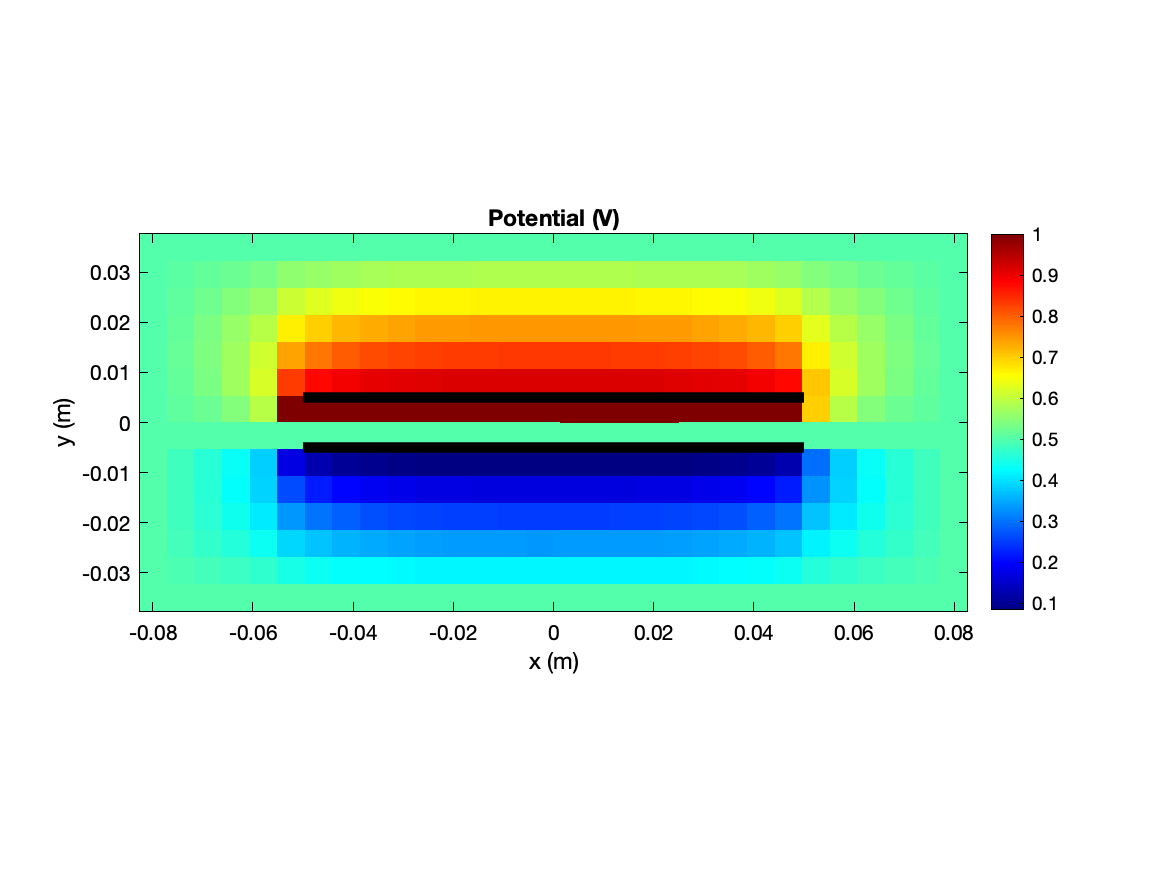
\includegraphics[width=\textwidth]{figures/coarse/potential_map.png}
        \caption{Potential map, $\delta = 0.005$ m.}
        \label{fig:potential_map_coarse}
    \end{subfigure}
    \hfill
    \begin{subfigure}[b]{0.48\textwidth}
        
\includegraphics[width=\textwidth]{figures/fine/potential_map.png}
        \caption{Potential map, $\delta = 0.002$ m.}
        \label{fig:potential_map_fine}
    \end{subfigure}
    \caption{Electric potential distribution. [COMMENTO: il potenziale deve essere 
    monotono tra le piastre, decadere regolarmente verso $\Gamma$, e non mostrare 
    oscillazioni. Discutere eventuali differenze tra le due mesh.]}
    \label{fig:potential_coarse}
\end{figure}

\begin{figure}[h!]
    \centering
    \begin{subfigure}[b]{0.48\textwidth}
        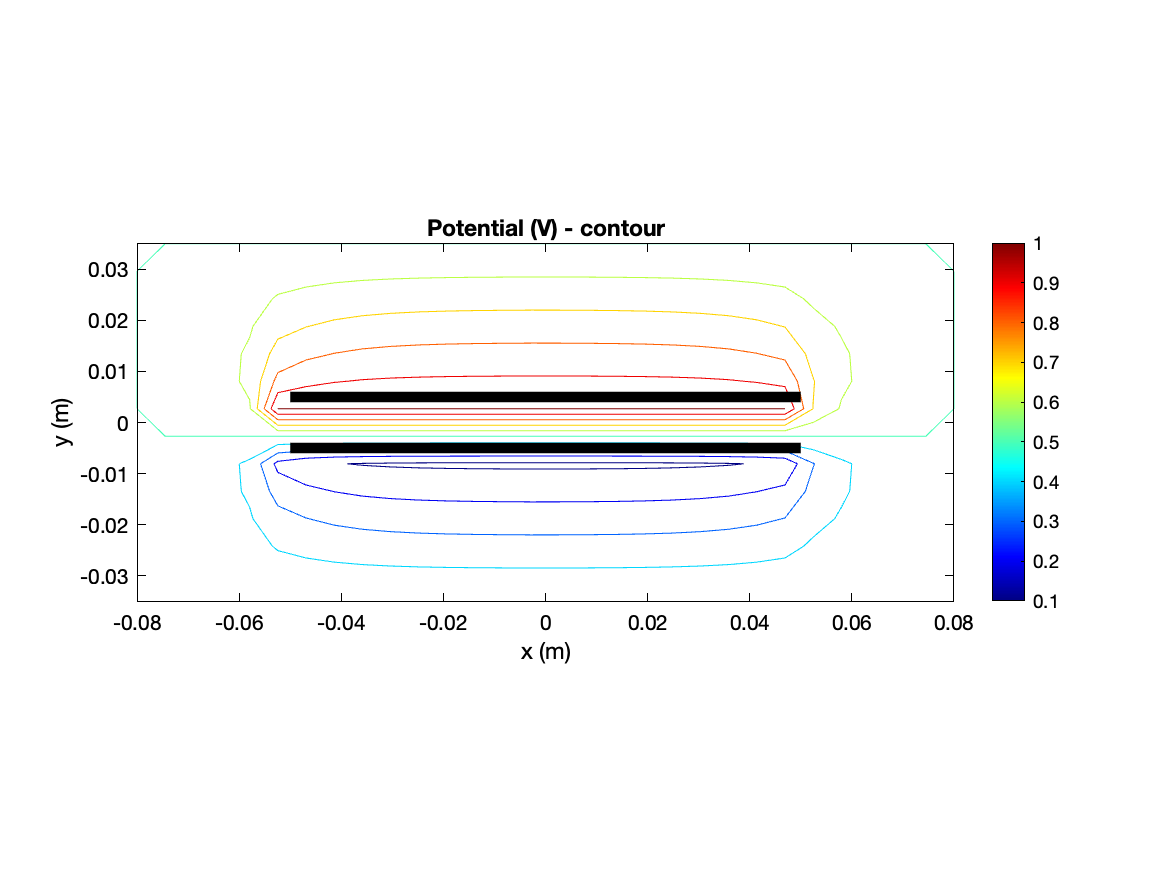
\includegraphics[width=\textwidth]{figures/coarse/potential_contour.png}
        \caption{Equipotential lines, $\delta = 0.005$ m.}
    \end{subfigure}
    \hfill
    \begin{subfigure}[b]{0.48\textwidth}
        
\includegraphics[width=\textwidth]{figures/fine/potential_contour.png}
        \caption{Equipotential lines, $\delta = 0.002$ m.}
    \end{subfigure}
    \caption{Equipotential lines. [COMMENTO: le linee devono essere orizzontali e 
    uniformemente spaziate al centro, e incurvarsi regolarmente ai bordi delle piastre 
    — questa è la firma visiva dei campi di frangia.]}
    \label{fig:potential_fine}
\end{figure}

% ------------------------------------------------------------------
\textbf{Electric field.}
Figures~\ref{fig:efield_coarse} and~\ref{fig:efield_fine} show the electric field 
magnitude and direction.

\begin{figure}[h!]
    \centering
    \begin{subfigure}[b]{0.48\textwidth}
        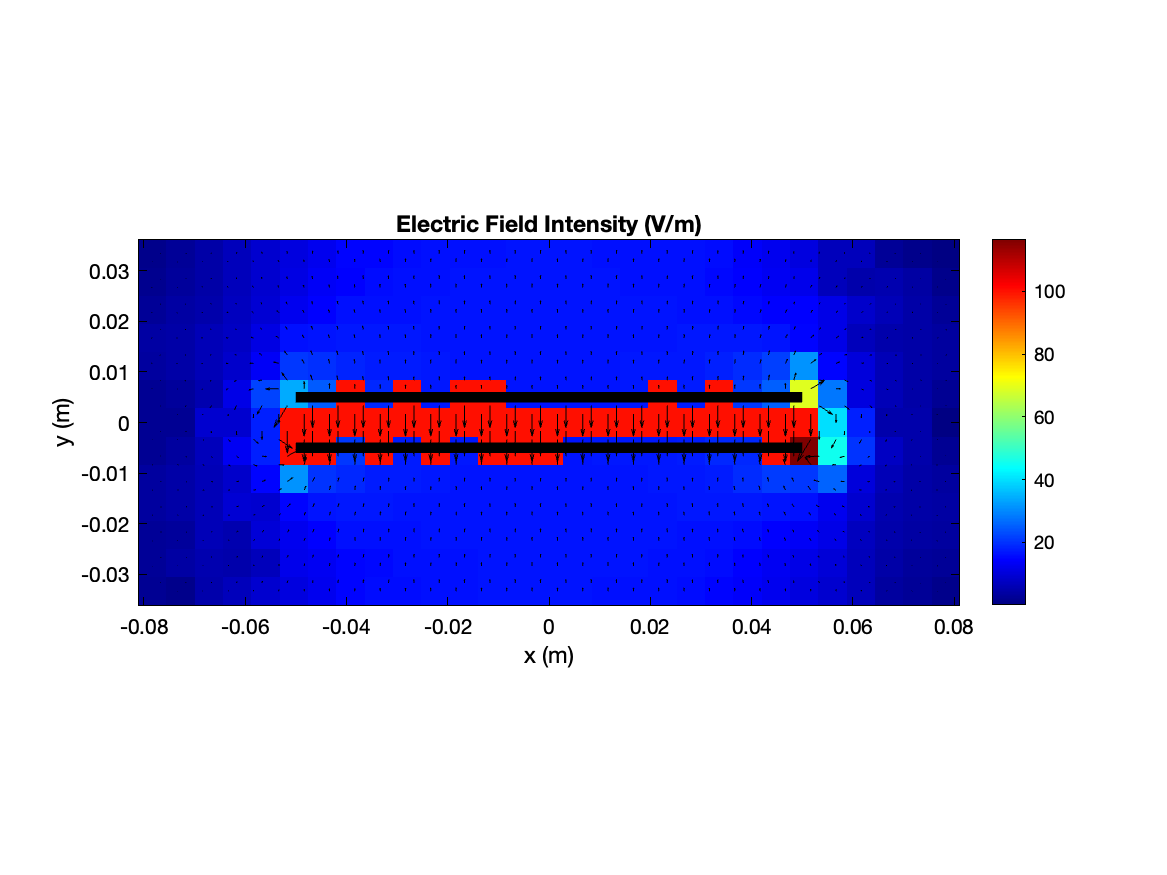
\includegraphics[width=\textwidth]{figures/coarse/efield_map.png}
        \caption{$\delta = 0.005$ m.}
    \end{subfigure}
    \hfill
    \begin{subfigure}[b]{0.48\textwidth}
        
\includegraphics[width=\textwidth]{figures/fine/efield_map.png}
        \caption{$\delta = 0.002$ m.}
    \end{subfigure}
    \caption{Electric field intensity and direction. [COMMENTO: al centro del 
    condensatore il campo deve essere uniforme e verticale, con $|\mathbf{E}| \approx 
    (V_1-V_2)/dy = 100$ V/m. Discutere la concentrazione di campo ai bordi delle 
    piastre e come migliora con la mesh più fine.]}
    \label{fig:efield_coarse}
\end{figure}

\begin{figure}[h!]
    \centering
    \begin{subfigure}[b]{0.48\textwidth}
        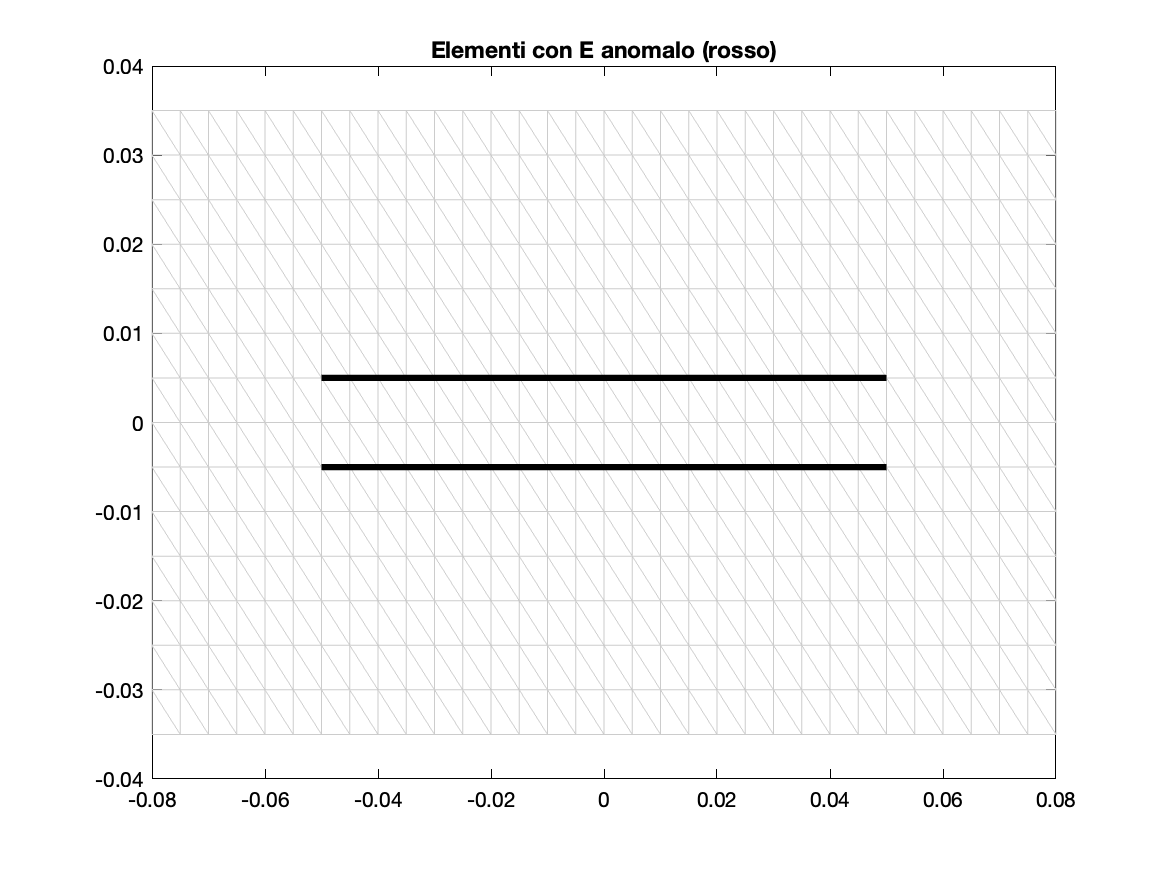
\includegraphics[width=\textwidth]{figures/coarse/bad_elements.png}
        \caption{$\delta = 0.005$ m.}
    \end{subfigure}
    \hfill
    \begin{subfigure}[b]{0.48\textwidth}
        
\includegraphics[width=\textwidth]{figures/fine/bad_elements.png}
        \caption{$\delta = 0.002$ m.}
    \end{subfigure}
    \caption{Elements with $|\mathbf{E}| > 50$ V/m highlighted in red. [COMMENTO: 
    verificare che gli elementi anomali siano localizzati solo agli angoli delle piastre 
    e che il loro numero non cresca con la raffinazione — se cresce indica un problema 
    nel coupling, se rimane costante è la singolarità fisica attesa.]}
    \label{fig:efield_fine}
\end{figure}

% ------------------------------------------------------------------
\textbf{Normal derivative on $\Gamma$.}

\begin{figure}[h!]
    \centering
    \begin{subfigure}[b]{0.48\textwidth}
        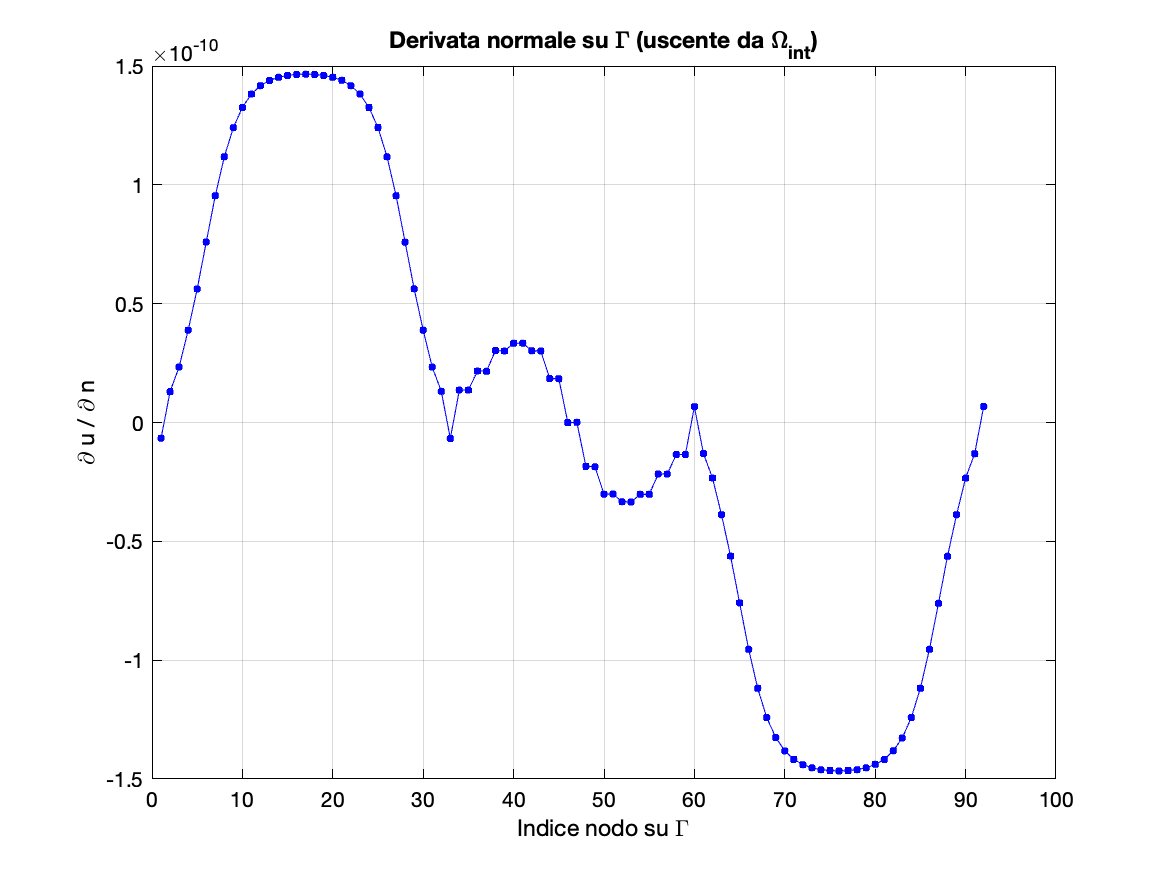
\includegraphics[width=\textwidth]{figures/coarse/q_gamma.png}
        \caption{$\delta = 0.005$ m.}
    \end{subfigure}
    \hfill
    \begin{subfigure}[b]{0.48\textwidth}
        
\includegraphics[width=\textwidth]{figures/fine/q_gamma.png}
        \caption{$\delta = 0.002$ m.}
    \end{subfigure}
    \caption{Normal derivative $\partial u / \partial n$ on $\Gamma$. [COMMENTO: 
    il flusso deve essere apprezzabile solo nella porzione di $\Gamma$ più vicina alle 
    piastre e trascurabile altrove. La somma totale deve essere prossima a zero per 
    la legge di Gauss — riportare il valore numerico di $\sum_i q_i$.]}
    \label{fig:q_gamma}
\end{figure}

% ------------------------------------------------------------------
\textbf{Surface charge density.}

\begin{figure}[h!]
    \centering
    \begin{subfigure}[b]{0.48\textwidth}
        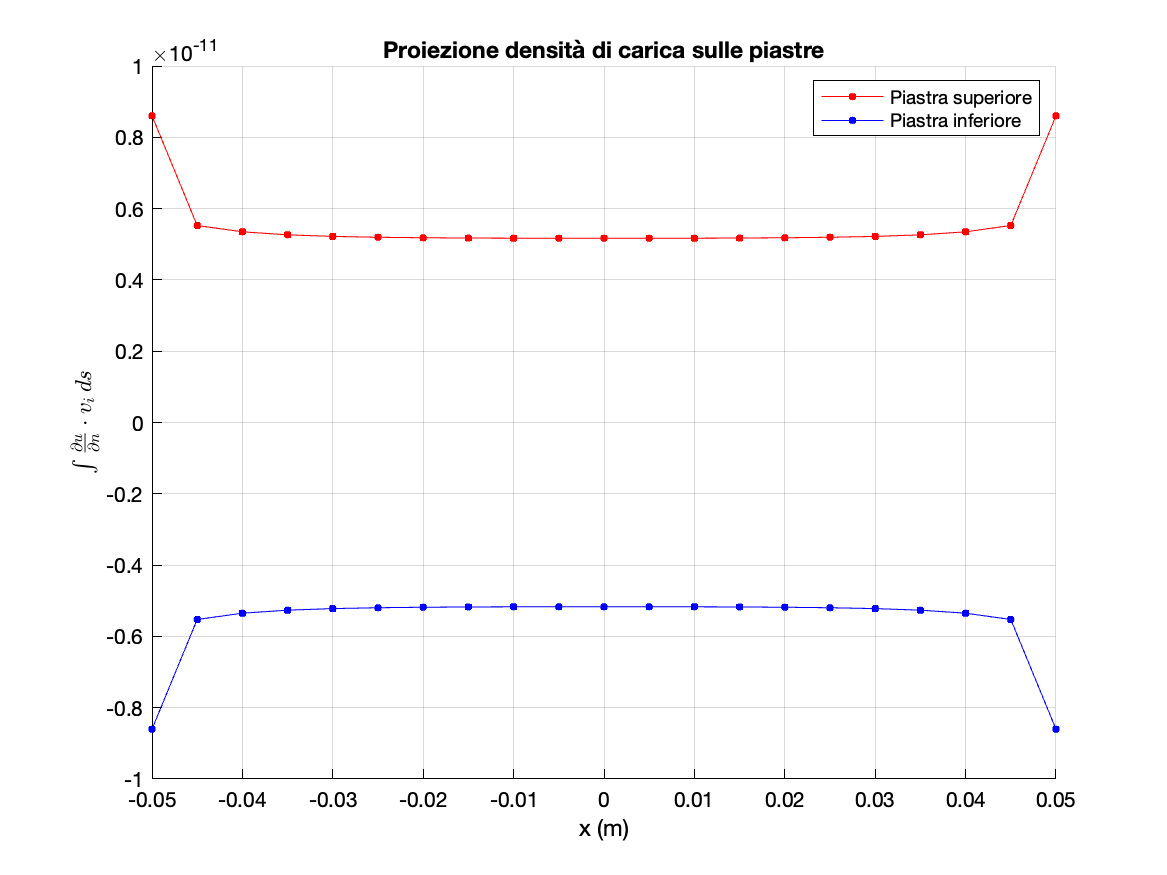
\includegraphics[width=\textwidth]{figures/coarse/charge_density.png}
        \caption{$\delta = 0.005$ m.}
    \end{subfigure}
    \hfill
    \begin{subfigure}[b]{0.48\textwidth}
        
\includegraphics[width=\textwidth]{figures/fine/charge_density.png}
        \caption{$\delta = 0.002$ m.}
    \end{subfigure}
    \caption{Projected surface charge density on the plates. [COMMENTO: la 
    distribuzione deve essere approssimativamente uniforme nella zona centrale e 
    crescere verso i bordi. Le due piastre devono avere distribuzioni di segno 
    opposto e uguale integrale — verificare la carica totale su ciascuna piastra.]}
    \label{fig:charge_density}
\end{figure}

% ------------------------------------------------------------------
\textbf{Capacitance}
Table~\ref{tab:capacitance} summarizes the capacitance values obtained with the two 
mesh levels.

\begin{table}[h!]
    \centering
    \begin{tabular}{lcccc}
        \hline
        Mesh & $\delta$ (m) & $C_{\text{full}}$ (pF/m) & 
        $C_{\text{clean}}$ (pF/m) & Error w.r.t. $C_{\text{ideal}}$ \\
        \hline
        Coarse & 0.005 & [VAL] & [VAL] & [VAL]\% \\
        Fine   & 0.002 & [VAL] & [VAL] & [VAL]\% \\
        \hline
        Ideal  & --    & 88.5  & 88.5  & -- \\
        \hline
    \end{tabular}
    \caption{Capacitance per unit length for the two mesh levels. $C_{\text{full}}$ 
    includes all elements; $C_{\text{clean}}$ excludes elements with 
    $|\mathbf{E}| > 50$ V/m near the plate edges. [COMMENTO: discutere la 
    convergenza tra le due mesh e il gap residuo rispetto al valore ideale, 
    attribuendolo ai campi di frangia.]}
    \label{tab:capacitance}
\end{table}


%% ------------------------------------------------------------

%% ------------------------------------------------------------
\section{Conclusions}

%% ------------------------------------------------------------

%% ------------------------------------------------------------
\section{Acknowledgements}

This report is based on Chapter 6 of the book \textit{Topics in Boundary Element Research} by C.A. Brebbia \cite{brebbia1990}. 
The implementation of the code derives, for the FEM part, from the work of Ozlem Ozgun and Mustafa Kuzuoglu \cite{ozgun2018}, distributed under the GNU General Public License, and for the BEM part, from code developed during the course \textit{Computational Electromagnetics} by Prof. Di Rienzo. 
Furthermore, artificial intelligence tools have been used in the preparation of this report. The full project code is available on GitHub: \url{https://github.com/Michelino21/FemBem_Project}.
%% ------------------------------------------------------------

%% ------------------------------------------------------------
\newpage
\bibliographystyle{unsrt}  % numerazione in ordine di citazione
\bibliography{references}  % il tuo file .bib si chiama references.bib
%% ------------------------------------------------------------

\newpage
\append{Introduzione Italiana}

Un classico esempio di accoppiamento FEM/BEM in un problema elettrostatico è il calcolo del campo elettrico generato da un condensatore a facce piane parallele. In una simulazione di questo tipo è spesso utile visualizzare non solo il comportamento del campo all’interno del condensatore, ma anche quello all’esterno. Nei corsi di Fisica 2, il campo esterno viene di norma assunto nullo; in realtà, a causa degli effetti di bordo, esso non è trascurabile e in alcune applicazioni può avere un ruolo rilevante. Questa è la motivazione principale per analizzare in maggiore dettaglio il comportamento del campo elettrico in un problema di questo tipo.

In questo progetto considereremo il caso relativamente semplice di un condensatore a facce piane parallele (si veda la figura di riferimento). Oltre alle cariche presenti sulle armature, non saranno considerate altre sorgenti nello spazio. L’equazione differenziale da risolvere è la prima legge di Maxwell ~\eqref{eq:prima_legge_maxwell} nella sua forma elettrostatica semplificata ~\eqref{eq:prima_legge_maxwell_semplificata}, trattata esprimendo il campo elettrico come gradiente del potenziale. ~\eqref{eq:prima_legge_maxwell_semplificata_potenziale}

\begin{equation}
	\nabla \cdot D = \rho
\label{eq:prima_legge_maxwell}
\end{equation}

\begin{equation}
	\nabla \cdot E = 0
\label{eq:prima_legge_maxwell_semplificata}
\end{equation}

\begin{equation}
	\Delta V = 0
\label{eq:prima_legge_maxwell_semplificata_potenziale}
\end{equation}

Un primo approccio ben noto consiste nell’utilizzare il metodo degli elementi finiti (FEM). Si definisce un dominio sufficientemente ampio da contenere il condensatore e si impone sul bordo un potenziale nullo, assumendo che a distanza sufficientemente grande il potenziale tenda effettivamente a zero. Questo metodo presenta tuttavia alcuni svantaggi: richiede domini molto estesi e quindi mesh di grandi dimensioni, con conseguente aumento dei tempi di calcolo. Inoltre la finezza della mesh deve essere omogenea dentro e fuori dal condensatore, anche se la qualità richiesta per ottenere un buon risultato non è la stessa nelle due regioni. Calcolare il campo esterno tramite FEM porta quindi a un significativo spreco computazionale e, in ogni caso, il potenziale non può essere rappresentato fino all’infinito, introducendo un’inevitabile approssimazione.

Il metodo BEM, invece, offre una soluzione più efficiente al problema. Riducendo di un ordine la dimensione del dominio, permette di ottenere notevoli vantaggi in termini computazionali. Per sua natura il BEM consente di calcolare con precisione la variabile incognita in qualsiasi punto interno a un dominio, risolvendo il problema solo sul suo bordo. (fig) Il BEM risulta applicabile anche a domini molto estesi o non limitati (fig.), a patto di conoscere a priori l’andamento asintotico del potenziale e che esso converga come $1/r^2$. In tali casi, il BEM riesce a rappresentare correttamente il comportamento all’infinito senza introdurre approssimazioni artificiali.

Lo scopo di questo lavoro è quindi combinare FEM e BEM per ottenere risultati più accurati a costi computazionali inferiori. L’idea è sfruttare il FEM per determinare con precisione la soluzione all’interno del condensatore e utilizzare il BEM per estenderla verso l’esterno fino all’infinito in modo esatto. Il meccanismo di accoppiamento tra i due metodi sarà descritto in dettaglio nella sezione dedicata.

\end{document}